\section{Gating Mechanisms – How Experts Are Selected}
\begin{frame}[allowframebreaks]{}
    \LARGE Gating Mechanisms – \textbf{How Experts Are Selected}
\end{frame}

\begin{frame}[allowframebreaks]{Gating Mechanisms – How Experts Are Selected}
    \begin{itemize}
        \item \textbf{Gating Mechanism:}
        \begin{itemize}
            \item A crucial component in Mixture of Experts (MoE) models determines which expert(s) to activate for a given input.
            \item Uses a learned function to compute a score for each expert.
            \item The scores are used to select the top-$k$ experts.
            \item (A small neural network that selects the top-k experts to use for a given input.)
        \end{itemize}
    \framebreak
        \item \textbf{How it works:}
        \begin{itemize}
            \item Input is passed through a gating network.
            \item The gating network outputs a probability distribution over experts.
            \item Only the experts with the highest probabilities are activated.
            \item This allows the model to focus on relevant experts for each input.
        \end{itemize}
    \framebreak
        \begin{itemize}
            \item \textbf{MoE Formulation}
            \begin{itemize}
                \item Input token: $x$
                \item Gating network $G$ calculates expert distribution.
            \end{itemize}

            \item \textbf{Gating Network Calculation}
            \begin{itemize}
                \item Linear transformation: $logits = W_g x$
                \item Softmax activation: $P = \text{softmax}(logits)$
                \item $W_g$: trainable weight matrix
                \item $P$: probability vector for each expert
            \end{itemize}
        \framebreak
            \item \textbf{Dense MoE Output}
            \begin{itemize}
                \item Output $y = \sum_{i=1}^N P_i E_i(x)$
                \item Combines all experts with weights $P_i$.
            \end{itemize}

            \item \textbf{Sparse MoE Goal}
            \begin{itemize}
                \item Focus on computational efficiency.
                \item Only activate a small subset of experts per token.
                \item Requires a mechanism to select experts based on $P$.
            \end{itemize}
        \end{itemize}
    \framebreak
        \begin{itemize}
            \item \textbf{Prevalent Strategy}
            \begin{itemize}
                \item For sparse MoEs, selects a subset of experts.
                \item Gating network chooses $k$ experts with highest probabilities.
                \item Typically, $k$ is small (e.g., 1 or 2).
            \end{itemize}
        \framebreak
            \item \textbf{Process Overview}
            \begin{itemize}
                \item \textbf{Compute Scores:} Calculate gating logits or probabilities ($P$).
                \item \textbf{Select Top-k:} Identify indices $I = \{i_1, i_2, \dots, i_k\}$ for top $k$ values in $P$.
                \item \textbf{Re-normalize Scores (Optional):}
                \begin{itemize}
                    \item $P_{sel}$: sub-vector of $P$ for selected indices $I$.
                    \item Re-normalized weights $P'$:
                    \[ P_j' = \frac{\exp(\text{logits}_{i_j})}{\sum_{l=1}^k \exp(\text{logits}_{i_l})} \quad \text{for } j=1 \dots k \]
                \end{itemize}
                \item \textbf{Compute Weighted Output:}
                \begin{itemize}
                    \item $y = \sum_{j=1}^k P_j' E_{i_j}(x)$
                    \item Uses (re-normalized) probabilities as weights.
                \end{itemize}
            \end{itemize}
        \framebreak
            \item \textbf{Choice of $\boldsymbol{k}$}
            \begin{itemize}
                \item $k=1$: Token routed to single expert.
                \begin{itemize}
                    \item Maximizes sparsity.
                    \item Limits knowledge combination.
                \end{itemize}
                \item $k=2$: Token uses two experts.
                \begin{itemize}
                    \item Balances sparsity and representational capacity.
                    \item Doubles computational cost vs. $k=1$.
                \end{itemize}
                \item $\boldsymbol{k}$ is a key hyperparameter affecting performance and cost.
            \end{itemize}
        \end{itemize}
    \framebreak
        \begin{figure}[h]
            \centering
            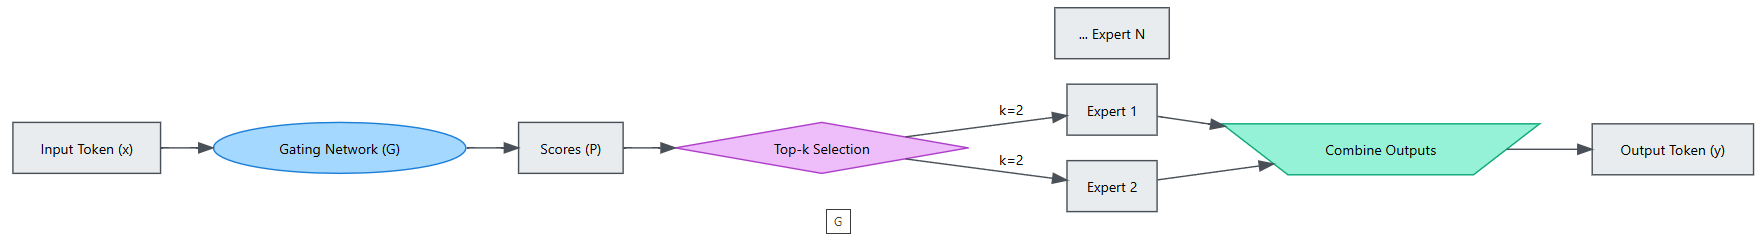
\includegraphics[width=\textwidth,height=0.8\textheight,keepaspectratio]{images/lrm+moe/gating-network.png}
            \caption*{Source: \href{https://apxml.com/courses/mixture-of-experts/chapter-2-advanced-moe-architectures/designing-gating-networks}{Designing Effective Gating Networks}}
        \end{figure}
    \end{itemize}
    \framebreak
        \begin{itemize}
            \item \textbf{Load-Balanced + Entropy-Regularized Gating}
            \begin{itemize}
                \item Ensures efficient and equal expert utilization.
                \item Prevents overloaded or underutilized experts.
                \item \textbf{Load-Balanced:}
                \begin{itemize}
                    \item Penalty in loss encourages even token distribution.
                    \item Avoids "expert collapse."
                \end{itemize}
                \item \textbf{Entropy-Regularized:}
                \begin{itemize}
                    \item Promotes diverse expert selection.
                    \item Nudges model to use full range of experts.
                \end{itemize}
            \end{itemize}
        \framebreak
            \item \textbf{Examples in Practice}
            \begin{itemize}
                \item \textbf{Example 1: Switch Transformer Gating}
                \begin{itemize}
                    \item Primarily uses \textbf{Top-1 routing}.
                    \item Incorporates \textbf{load balancing penalty}.
                    \item Ensures experts are actively learning and distributed.
                \end{itemize}
                \item \textbf{Example 2: MoE-LLaMA}
                \begin{itemize}
                    \item Employs \textbf{Top-2 gating}.
                    \item \textbf{Avoids token dropout}.
                    \item Aims for smoother and consistent performance.
                \end{itemize}
            \end{itemize}
        \end{itemize}
\end{frame}